% YOUR SOLUTION TO PROBLEM 2 GOES HERE
% THE LATEX CODE YOU PUT HERE WILL BE INLINED (IF YOU NEED ADD ANY PACKAGES DO IT IN THE MAIN TEMPLATE FILE)


Since $L$ is regular, there is a DFA $M$ that can match $L$. Let us create an NFA $M'$ that can match $L^R$, which will prove that $L^R$ is regular.
$M'$ is composed of all of $M$'s states, plus one new state. This new state is the start state of the NFA, and it contains only $\epsilon$ transitions to all states that were accepting states of $M$. The accepting state of $M'$ is the start state of $M$. The transition function of $M'$ is the opposite of $M$; if an input $x$ caused $M$ to go from $q_0$ to $q_1$, it causes $M'$ to go from $q_1$ to $q_0$.

To express it more formally:
\begin{align*}
M &= (Q, \Sigma, \delta, s, F) \\
M' &= (Q', \Sigma, \delta;, s', F') \\
s' &= \text{new state, connected to the end of all the states }F \\
Q' &= Q + \{ s' \} \\
F' &= \{ s \} \\
\delta' &= \delta^R \\
\delta'(q,x) &= \left\{ 
  \begin{array}{l l}
    F & \quad \text{if } q = s' \\
    \{q_2 | \delta(q_2,x)\} = q & \quad \text{otherwise}
  \end{array} \right.
\end{align*}

%\begin{figure}[H]
%\centering
%\begin{tikzpicture}[shorten >=2pt, auto, node distance=2 cm, scale = 1, transform shape]
%    
%\node[state, initial] (q0) {$q_0$};
%\node[state] (anon0) [right of=q0, xshift=0.3cm, yshift=0.4cm] {};
%\node[state] (anon1) [right of=q0, xshift=1.3cm, yshift=-0.8cm] {};
%\node[state] (anon2) [right of=q0, xshift=1.7cm, yshift=1.5cm] {};
%\node[state, accepting] (anon3) [right of=q0, xshift=3.3cm, yshift=1.8cm] {};
%\node[state, accepting] (anon4) [right of=q0, xshift=2.9cm, yshift=-0.8cm] {};
%\node[draw=none,fill=none] (inv1)[right of=q0, yshift=1.3cm]{};
%\node[draw=none,fill=none] (inv2) [right of=q0, yshift=-1.3cm]{};
%\node [draw=black, fit = (anon0)(anon1)(anon2)(anon3)(anon4), inner sep=0.50cm]{};
%
%\path[->] (q0) edge node [align=center] {} (inv1);
%\path[->] (q0) edge node [align=center] {} (inv2);
%
%\end{tikzpicture}
%\caption{DFA $A_1$}
%\end{figure}
%
%
%\begin{figure}[H]
%\centering
%\begin{tikzpicture}[shorten >=2pt, auto, node distance=2 cm, scale = 1, transform shape]
%    
%\node[state, accepting] (q0) {};
%\node[state] (anon0) [right of=q0, xshift=0.3cm, yshift=0.4cm] {};
%\node[state] (anon1) [right of=q0, xshift=1.3cm, yshift=-0.8cm] {};
%\node[state] (anon2) [right of=q0, xshift=1.7cm, yshift=1.5cm] {};
%\node[state] (anon3) [right of=q0, xshift=3.3cm, yshift=1.8cm] {};
%\node[state] (anon4) [right of=q0, xshift=2.9cm, yshift=-0.8cm] {};
%\node[state, initial] (s0) [right of=q0, xshift=8cm]{$q'_0$};
%
%\node[draw=none,fill=none] (inv1)[right of=q0, yshift=1.3cm]{};
%\node[draw=none,fill=none] (inv2) [right of=q0, yshift=-1.3cm]{};
%\node [draw=black, fit = (anon0)(anon1)(anon2)(anon3)(anon4), inner sep=0.50cm]{};
%
%\path[<-] (q0) edge node [align=center] {} (inv1);
%\path[<-] (q0) edge node [align=center] {} (inv2);
%\path[<-] (q0) edge node [align=center] {} (inv1);
%\path[<-] (q0) edge node [align=center] {} (inv2);
%
%\end{tikzpicture}
%\caption{DFA $A_1$}
%\end{figure}


\begin{figure}[H]
\centering
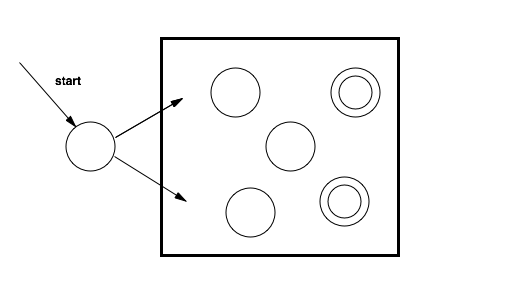
\includegraphics[scale=0.6]{original_dfa}
\caption{Original DFA $M$}
\end{figure}


\begin{figure}[H]
\centering
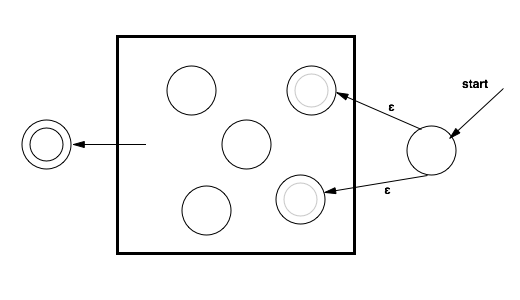
\includegraphics[scale=0.6]{NFA}
\caption{New NFA $M'$}
\end{figure}


This new machine $M'$ will be able to read every word the original machine $M$ was able to read, in the opposite direction; indeed, for every word $M$ was able to read it ended up in one of the accepting states to which $M'$ can transition to at no cost ($\epsilon$) from the start and therefore will end up after the reverse read of the word in the initial state of $M$, meaning in the accepting state of $M'$.


